\appendix

\chapter{Experiment Videos} \label{A:ExperimentVideos}
\section{Physical experiment}
A video of a physical laboratory experiment can be found here: \href{https://youtu.be/hxrZh7bj16A}{Physical Experiment}.

\section{Simulated Experiment}
A video of a simulated experiment can be found here: \href{https://youtu.be/po9pRVNtn78}{Simulation Experiment}.

\section{TurtleBot3 Simulated Experiment}
A video of a simulated experiment using a TurtleBot3 simulation can be found here: \href{https://youtu.be/_Dy3rSTHWYo}{TurtleBot3 Simulation Experiment}.

\chapter{Code} \label{A:Code}
\section{Mobile Robot \& Top-Level} \label{A:Code:uiaHusky0776}
Code for the mobile robot and to level system is provided in the public GitHub repository: \href{https://github.com/orjano-max/uia_husky_0776}{uia\_husky\_0776}.

\section{Pick and Place}\label{A:Code:uiaHuskyVx300}
Code for the pick and place system is provided in the public GitHub repository: \\\href{https://github.com/orjano-max/uia_husky_vx300}{uia\_husky\_vx300}.


\chapter{Technical Specification Tables}
Technical specification tables regarding some of the component used during the course of this project is provided in this chapter.
\section{Clearpath - Husky A200 Specs} 
\begin{table}[H]
\centering
\caption{Technical specifications for the Clearpath Husky A200, complete data sheet available in appendix \ref{A:fig:husky_data_sheet}, from \cite{clearpath_husky_website}}
\label{tab:husky:a200:specs}
\vspace{1mm}
\begin{tabular}{ll}
\hline
\multicolumn{2}{c}{\textbf{Husky A200 Specifications}}                                                            \\ \hline
Drivers and APIs                            & ROS, ROS 2, C++ and Python                                          \\
Wheel encoders                              & Quadrature: 78,000 {[}pulses/m{]}
        \\
Communication                               & RS232@115200 Baud                                                   \\
Battery                                     & \begin{tabular}[c]{@{}l@{}}12V 20Ah\\ Sealed Lead Acid\end{tabular} \\
\multicolumn{1}{c}{User Power Distribution} & \begin{tabular}[c]{@{}l@{}}5V 5A\\  12V 5A\\  24V 5A\end{tabular}   \\
Weight                                      & 50 {[}kg{]}                                                         \\
Payload Capacity                            & 75 {[}kg{]}                                                         \\
External Dimensions                         & 990 x 670 x 390 {[}mm{]}                                            \\ \hline
\end{tabular}
\end{table}

\section{Interbotix - VX300 Specs}
\begin{table}[H]
\centering
\caption{Technical Specifications for the Interbotix VX300 Manipulator. From \cite{interbotix_vx300}}
\label{tab:M:CD:FC:VX300Specs}
\vspace{1mm}
\begin{tabular}{ll}
\hline
\multicolumn{2}{c}{\textbf{Interbotix VX300 Specifications}} \\ \hline
Degrees of Freedom               & 5                         \\
Reach                            & 750{[}mm{]}               \\
Span                             & 1500{[}mm{]}              \\
Accuracy                         & 5-8{[}mm{]}               \\
Working Payload                  & 750{[}g{]}                \\ \hline
\end{tabular}
\end{table}

% \begin{figure}[H]
%   \centering
%   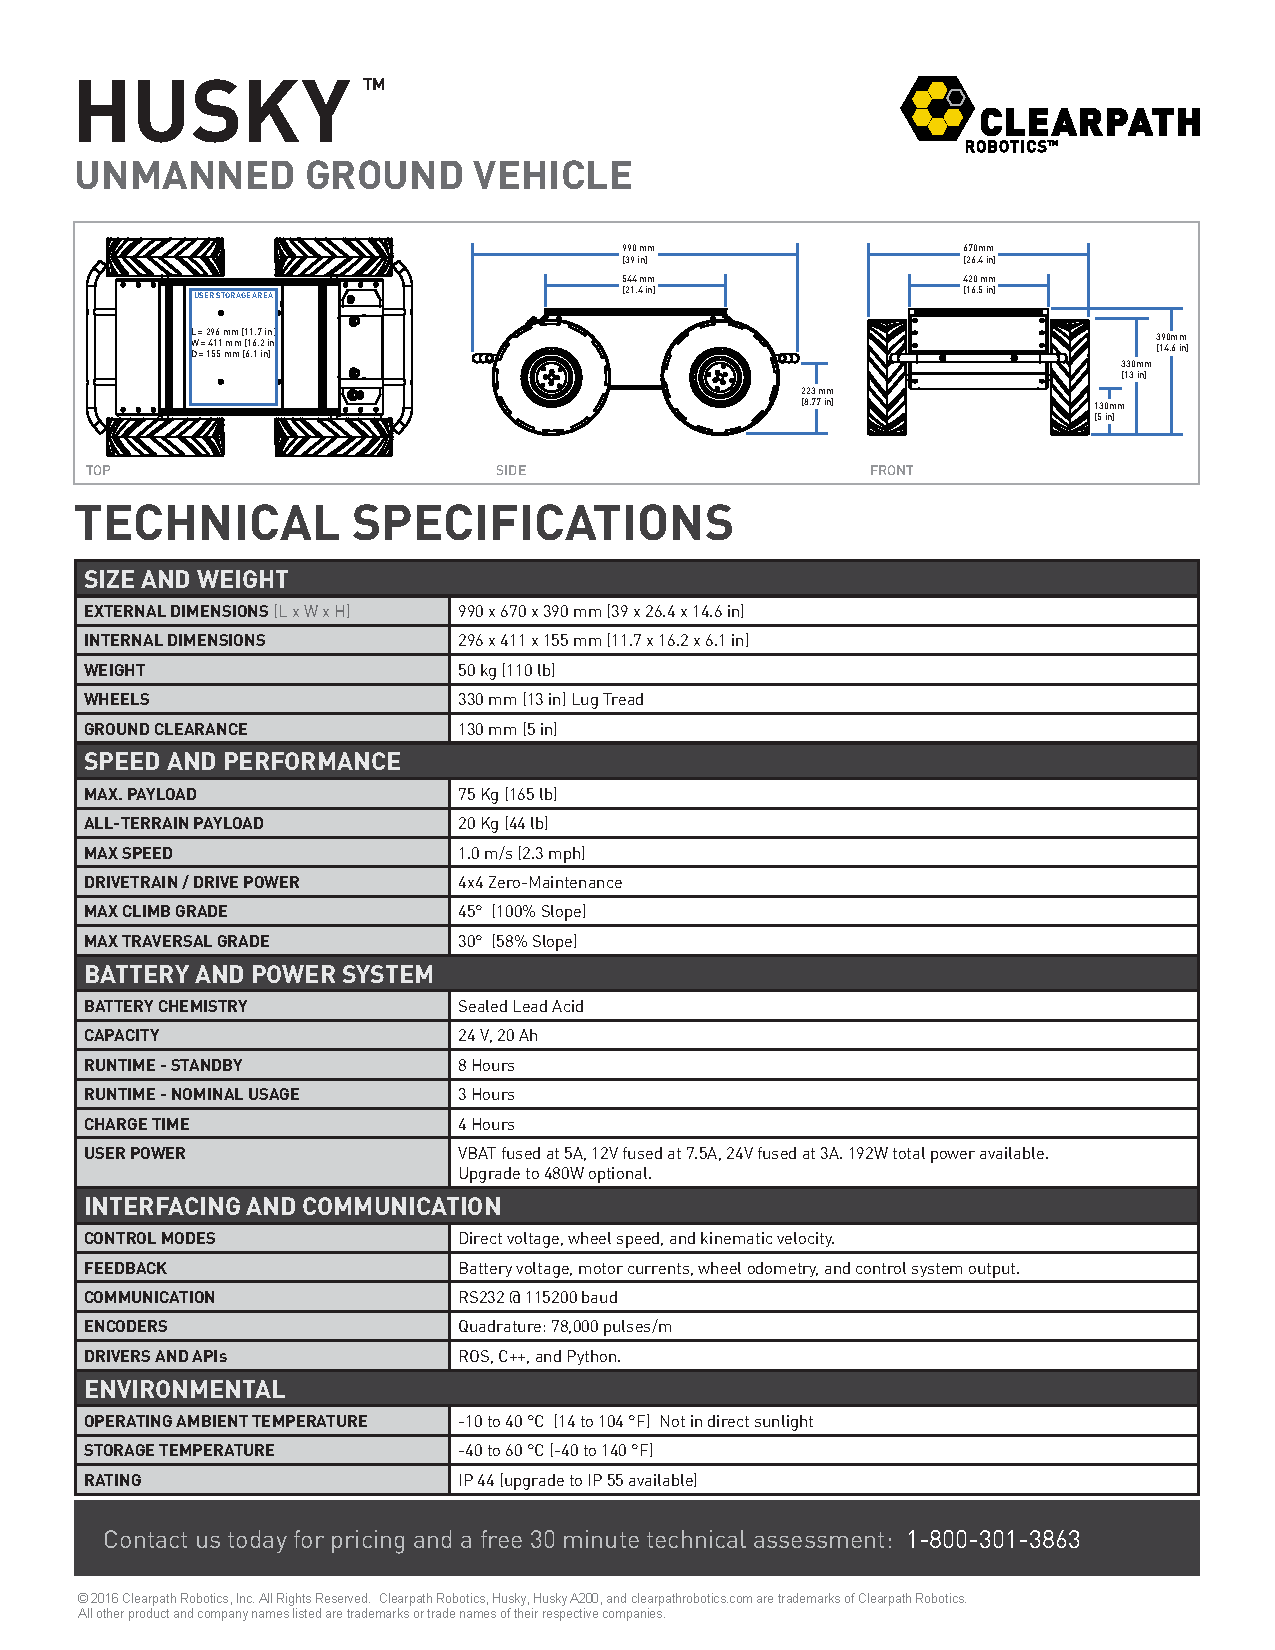
\includegraphics[width = 0.9\textwidth]{appendices/HUSKY_DATA_SHEET_Jan22.pdf}
% \end{figure}

\chapter{Drawings}
This chapter provides a general arrangement drawing and an electrical interface drawing of the robotic system.
\section{General Arrangement}\label{A:D:GeneralArrangement}
A general arrangement drawing describing the physical arrangement of all the components mounted on the UGV is presented in figure \ref{fig:general_arrangement}.

\begin{figure}[htp]
  \centering
   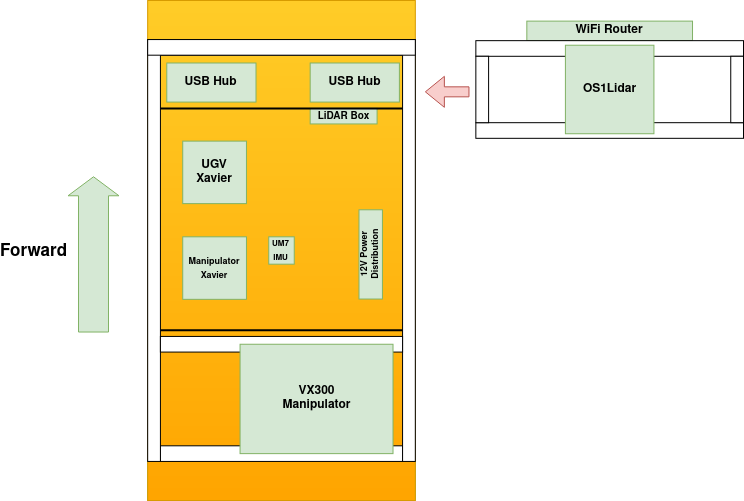
\includegraphics[width=0.9\textwidth]{Figures/general_arrangement.drawio.png}
  \caption{General arrangement drawing of UGV platform. Here, the physical position of different hardware components are defined. The sensor frame is drawn to the left of the main frame.}
  \label{fig:general_arrangement}
\end{figure}
%aj only of figure for a subsection. doesn't look good - I DIDNT UNDERSTAND THIS - ØØ

\section{Electrical Interface}\label{A:ElectricalInterface}
The different components in the system is powered through the user power supply of the UGV(see table \ref{tab:husky:a200:specs}). Figure \ref{fig:circuit_diagram} is a circuit diagram that illustrates the DC power distribution.
\begin{figure}[htp]
  \centering
  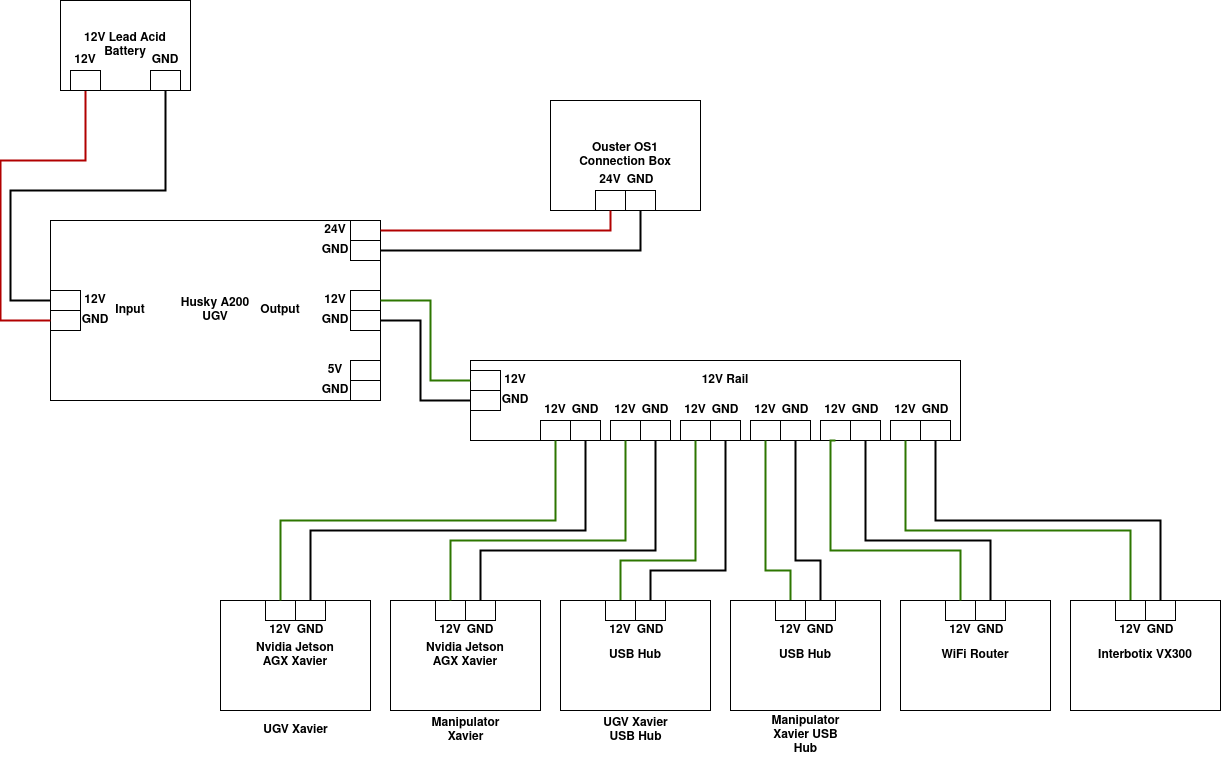
\includegraphics[angle=-90, width = 0.9\textwidth]{Figures/circuit_diagram.drawio.png}
  \caption{Circuit diagram showing the power distribution on the UGV}
  \label{fig:circuit_diagram}
\end{figure}

% \chapter{Implementation of Scene Publisher} \label{A:lst:ScenePublisher}
% \UseRawInputEncoding
% \lstinputlisting[language=C++]{code/src/scene_geometry_publisher/src/scene_geometry_publisher.cpp}

\chapter{UML Class Diagrams}
UML Class diagrams explaining classes made during the course of the project.

\section{Scene Publisher UML}
\begin{figure}[H]
  \label{A:fig:scenePublisherUML} 
  \centering
  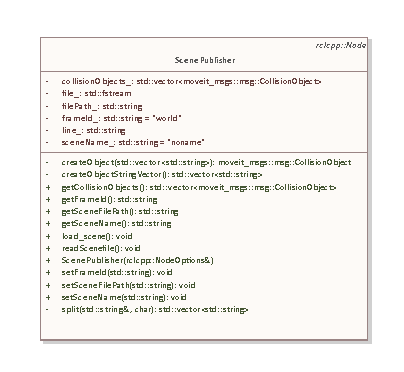
\includegraphics[width = 0.98\textwidth]{Figures/scene_geometry_publisher.pdf}
  \caption{UML Class Diagram of the Scene Geometry publisher Node.}
\end{figure}

\section{Pick and PLace UML}
\begin{figure}[H]
  \centering
  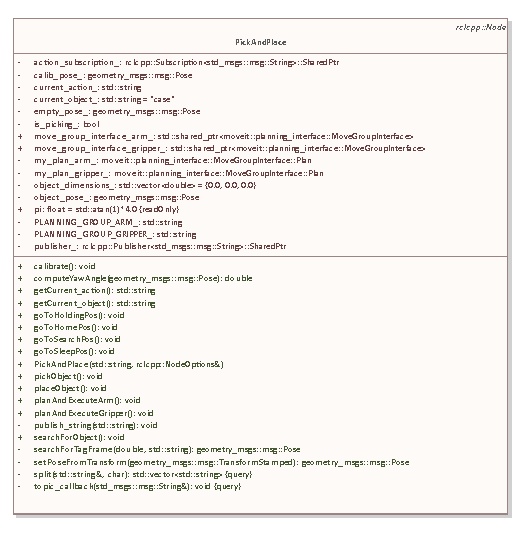
\includegraphics[width = 0.8\textwidth]{Figures/husky_pick_and_place.pdf}
  \caption{UML Class Diagram of the Husky Pick and Place Node.}
  \label{A:fig:PickAndPlaceUML}
\end{figure}

\section{Husky Master Node UML}

\begin{figure}[H]
  \centering
  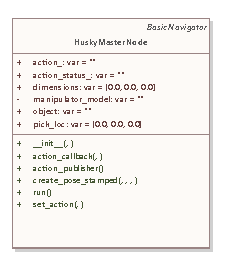
\includegraphics[width = 0.6\textwidth]{Figures/husky_master.pdf}
  \caption{UML Class Diagram of the Husky Master Node. As this is one class and interacts through ROS topics, it appears alone in the class diagram.}
  \label{A:fig:M:TL:huskyMasterUML}
\end{figure}

\chapter{Localisation Methods}
A more in depth explanation of Kalman Filter Localisation and Monte Carlo Localisation is presented in this chapter.
\section{Kalman Filter Localisation} \label{A:KalmanFilterLocalisation}
Figure \ref{fig:kalmanFilter} is an illustration from \cite{SiegwartRoland2011Itam} that demonstrates Kalman Filter localisation working principle. The robot is represented in a one-dimensional environment and it's positioning belief, $bel(x)$, is represented as a Gaussian distribution. From figure \ref{fig:kalmanFilter} \textit{(a)}, the robots initial is represented as a fairly confident Gaussian. The robot then moves, and in figure \ref{fig:kalmanFilter} \textit{(b)} the robot has estimated its position using it's wheel odometry. Since odometry accumulates measurement errors, it's belief is now represented as a less confident Gaussian. Next, the robot uses its perception system and sees that it is near the second pillar. This results in a posterior probability $p(z_t | x_t,M)$ of the observation represented as a Gaussian in figure \ref{fig:kalmanFilter} \textit{(c)}. The posterior observation is then fused with the robots belief after moving (fig. \ref{fig:kalmanFilter}\textit{(b)} and represented as $bel(x)$ in figure \ref{fig:monteCarloLocalisation}\textit{(c)}. It can be seen that this belief is more confident(narrower) than the two Gaussians it is comprised of. This makes sense since the two independent measurements agree and that would result in a more certain estimate. In the last step, seen in figure \ref{fig:kalmanFilter}\textit{(d)}, the robot has moved again and convolved its odometry with the previous belief. Because of the uncertainty of the odometry, the resulting belief is less confident.

\begin{figure}[htp]
  \centering
  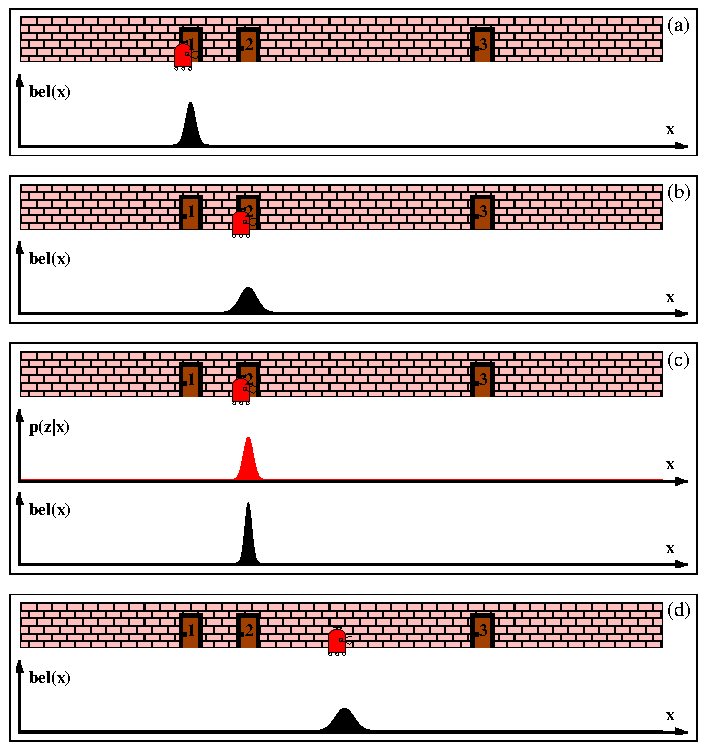
\includegraphics[width = 0.7\textwidth]{Figures/figKalmanFilter.pdf}
  \caption{Kalman Filter demonstration in a one-dimensional environment. Each figure, \textit{(a), (b), (c), (d)} represents a robot and it's positional belief $bel(x)$ as a Gaussian distribution. \textbf{(a):} The robots initial belief. \textbf{(b):} The robots belief after moving and convolving odometry with initial belief. \textbf{(C):} The robot observed the second pillar and gained a posterior probability $p(z|x,M)$. Fusing this with the belief from \textbf{(b)} results in a narrower belief $bel(x)$. \textbf{(d)} Robots belief after moving again and convolving the odometry with the previous belief. Figure from \cite{ThrunSebastian2005Pr}}
  \label{fig:kalmanFilter}
\end{figure}

\section{Monte Carlo Localisation} \label{A:MonteCarloLocalisation}
Figure \ref{fig:monteCarloLocalisation} is used to better explain how MCL works. The figure and description is adapted from \cite{ThrunSebastian2005Pr}. The figure illustrates a robot in a one-dimensional corridor. The belief $bel(x)$ is represented as pose particles with a height corresponding to their importance factor, hence the particle filter definition. In figure \ref{fig:monteCarloLocalisation}\textit{(a)} the global uncertainty is illustrated through a set of pose particles drawn at random and uniformly over the entire pose space. The robot could be anywhere in the corridor. Then, the robot senses the door and gives a posterior probability $p(z|x)$. MCL gives a importance factor to each particle from the initial particle sampling. The resulting belief$b(x)$ along with $p(z|x)$ can be seen in figure \ref{fig:monteCarloLocalisation}\textit{(b)}. In figure \ref{fig:monteCarloLocalisation}\textit{(c)} the robot has re-sampled the particle set and implemented its movement. It can be seen that the particles are now more densely populated around the most likely poses, but with uniform importance factors. The robot then senses another door and gives the posterior probability $p(z|x)$ again. Looking at figure \ref{fig:monteCarloLocalisation}, it is worth noticing that the posterior probability from \textit{(b)} and \textit{(d)} is equal, as the door sensor won't know the difference between each door. MCL again gives importance factors to each particle, as seen in the belief $bel(x)$ in figure \ref{fig:monteCarloLocalisation}\textit{(d)}. This time, most of the total particle mass is centred around the second door, which is also the robots position according to the illustration. In figure \ref{fig:monteCarloLocalisation}\textit{(e)}, the robot has moved and re-sampled the pose particles, which is centred around the most likely pose of the robot.

\begin{figure}[htp]
  \centering
  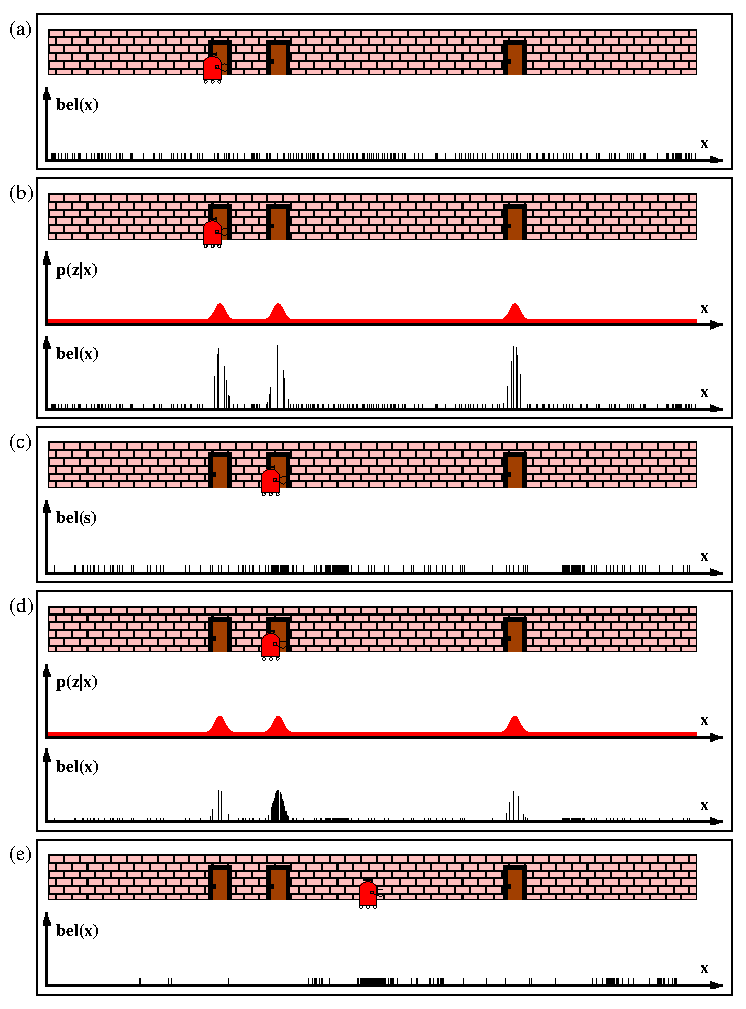
\includegraphics[width = 0.7\textwidth]{Figures/figMCL.pdf}
  \caption{Monte Carlo Localisation a one-dimensional environment. Figure from \cite{ThrunSebastian2005Pr}.}
  \label{fig:monteCarloLocalisation}
\end{figure}

\chapter{Path Planning Algorithms}
A more in depth explanation of Djikstra's Algorithm and A* path planning algorithms is explained in this chapter.
\section{Djikstra's Algorithm}\label{A:T:AN:PP:DjikstrasAlgotihm}
Djikstra's algorithm is a planning algorithm published by E. W. Djikstra in 1959\cite{DijkstraE.W1959Anot}. The algorithm presents a way to find the shortest path from a starting point $P_s$ to a goal $P_g$. This is done by giving a cost to the path it finds from $P_s$ to each node in the map, it will keep the paths with the lowest cost and keep searching until it has found the lowest cost path from $P_S$ to all nodes in the map. For each iteration, the algorithm will explore the unexplored node with the lowest calculated cost. The cost is usually based on distance or time taken to traverse the edge. In mobile robotics, the algorithm is often computed from the $P_g$, meaning that it will find the shortest path to any $P_s$ in the map. Thus, the robot is able to plan the best path to the goal based on it's current position without running the planning algorithm again \cite{SiegwartRoland2011Itam}. For example, if the robot is moving towards the goal and needs to take evasive actions because of some moving obstacle in it's trajectory. Time complexity for this algorithm is noted as $O(n\log(n)+m)$ where $n$ is the number of nodes and $m$ is the number of edges\cite{SiegwartRoland2011Itam}. See \cite{DijkstraE.W1959Anot} and \cite{SiegwartRoland2011Itam} for more information about the algorithm. 

\section{A* Algorithm}\label{A:T:AN:PP:A*Algorithm}
The A* algorithm is similar to Djikstra's algorithm in that it will give the edges between the nodes a cost. However A* also carries a heuristic which estimates the distance from explored nodes to the goal, $P_g$. For mobile robotics, this heuristic is often calculated as the distance between any cell and the goal cell, $p_g$ in the absence of obstacles (straight distance) \cite{SiegwartRoland2011Itam}. This way, the algorithm will usually explore nodes located in the direction towards the goal before expanding in any other direction. Because of this, the algorithm is often much faster than for example Djikstra's, but it is not guaranteed that the lowest cost path is found. The time complexity of this algorithm is also largely dependent on the weighting of the heuristic and the geometry of the map. See \cite{SiegwartRoland2011Itam} for a more in-depth explanation of the algorithm.

% \chapter{MAS531 - Autonomous Lane Keeping for UGV Using a Monocular Vision System and Machine Learning} \label{A:MAS513Report}

% \includepdf[pages=-]{appendices/MAS513_Project__Husky_Group.pdf}



